\section{Corridas de ejecución}

\subsection{Servidor ejecución}

El archivo donde se inicia la ejecución del servidor es \texttt{ServidorApplication.java}. Este archivo contiene el método \InlineCode{main} que se encarga de inicializar el servidor, configurar la base de datos y poner a disposición los servicios necesarios para que los clientes puedan conectarse y realizar operaciones.

En la consola muestra los \texttt{logs} de inicio, esto se aprecian en la Figura \ref{fig:logs-servidor}. Los \texttt{logs} muestran información sobre la configuración del servidor, la inicialización de la base de datos y la disponibilidad de los servicios.

\begin{figure}[H]
    \centering
    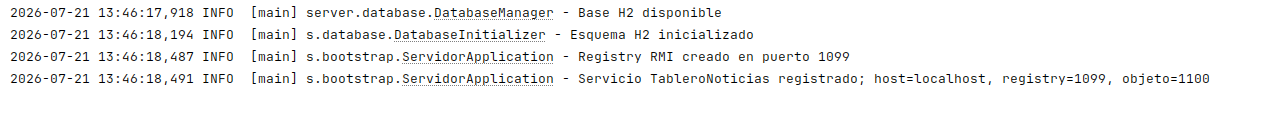
\includegraphics[width=1\textwidth]{assets/img/servidor/inicio.png}
    \caption{Logs de inicio del servidor}
    \label{fig:logs-servidor}
\end{figure}

\emph{No se necesito configurar nada adicional para que el servidor funcione, ya que las sentencias SQL para crear las tablas necesarias se ejecutan automáticamente al iniciar el servidor. Esto significa que no es necesario ejecutar ningún script adicional para configurar la base de datos.}

\subsection{Cliente ejecución}

El archivo donde se inicia la ejecución del cliente es \texttt{ClienteApplication.java}. Este archivo contiene el método \InlineCode{main} que se encarga de inicializar la interfaz gráfica, establecer la conexión con el servidor y permitir a los usuarios interactuar con la aplicación.

Si el servidor no esta activado y el cliente arranca en automático se muestra una ventana para que el usuario ingrese la dirección y el puerto correctos, como se muestra en la Figura \ref{fig:conexion-dialog}. Una vez conectado, el cliente puede enviar solicitudes al servidor y recibir respuestas, permitiendo a los usuarios interactuar con la aplicación de manera efectiva.

\begin{figure}[H]
    \centering
    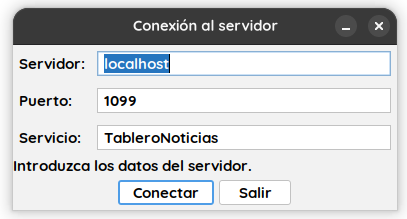
\includegraphics[width=0.4\textwidth]{assets/img/cliente/credenciales-servidor.png}
    \caption{Ventana de conexión del cliente}
    \label{fig:conexion-dialog}
\end{figure}

En caso de éxito o que las credenciales sean correctas, se muestra la ventana principal del cliente, como se muestra en la Figura \ref{fig:cliente-ventana-principal}. Esta ventana permite a los usuarios ver las noticias, iniciar sesión, cerrar sesión y publicar noticias (si se ha iniciado sesión).

\begin{figure}[H]
    \centering
    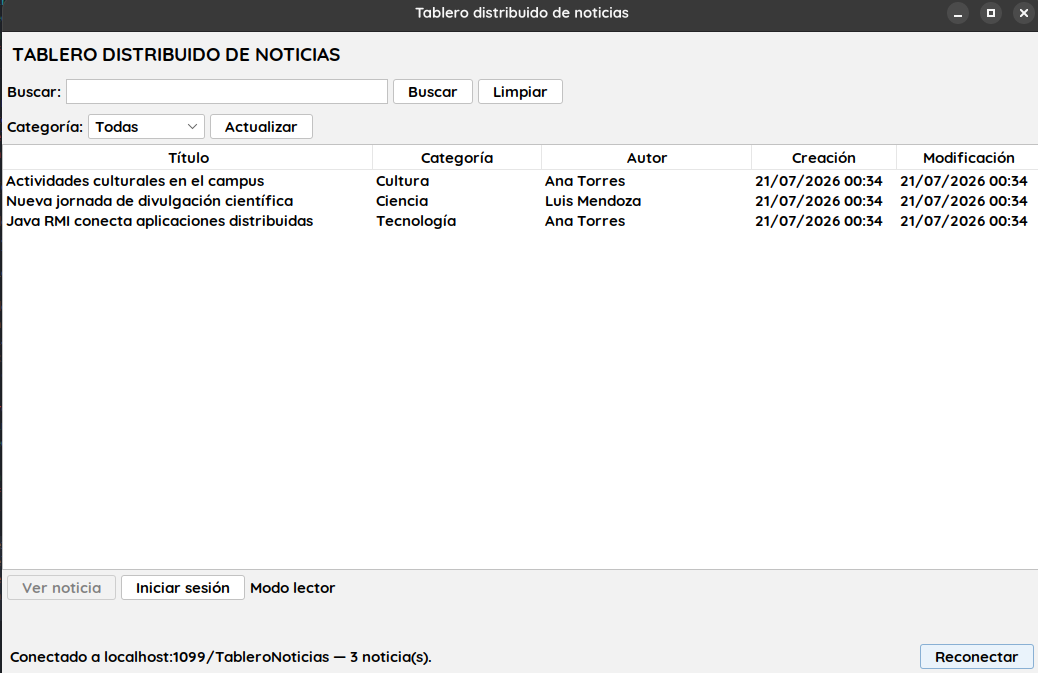
\includegraphics[width=0.8\textwidth]{assets/img/cliente/tablero-principal.png}
    \caption{Ventana principal del cliente}
    \label{fig:cliente-ventana-principal}
\end{figure}

Aquí el usuario sin necesidad de \texttt{iniciar sesión} puede ver las noticias publicadas, pero si desea publicar una noticia debe iniciar sesión con un usuario registrado. En caso de que el usuario no tenga una cuenta, debe solicitar al administrador del sistema que le cree una cuenta para poder iniciar sesión y publicar noticias.

Las funciones básicas de este apartado son las siguientes:

\begin{itemize}
    \item \textbf{Ver noticias:} Permite a los usuarios ver las noticias publicadas sin necesidad de iniciar sesión.
    \item \textbf{Iniciar sesión:} Permite a los usuarios registrados iniciar sesión en la aplicación para poder publicar noticias.
    \item \textbf{Cerrar sesión:} Permite a los usuarios buscar una noticia por su título usando el campo de búsqueda, tal y como se aprecia en la Figura \ref{fig:cliente-ventana-busqueda}, donde filtro por el término \emph{Java}.
    \item \textbf{Publicar noticias:} Permite a los usuarios filtrar por categoría, fecha o autor.
\end{itemize}

\begin{figure}[H]
    \centering
    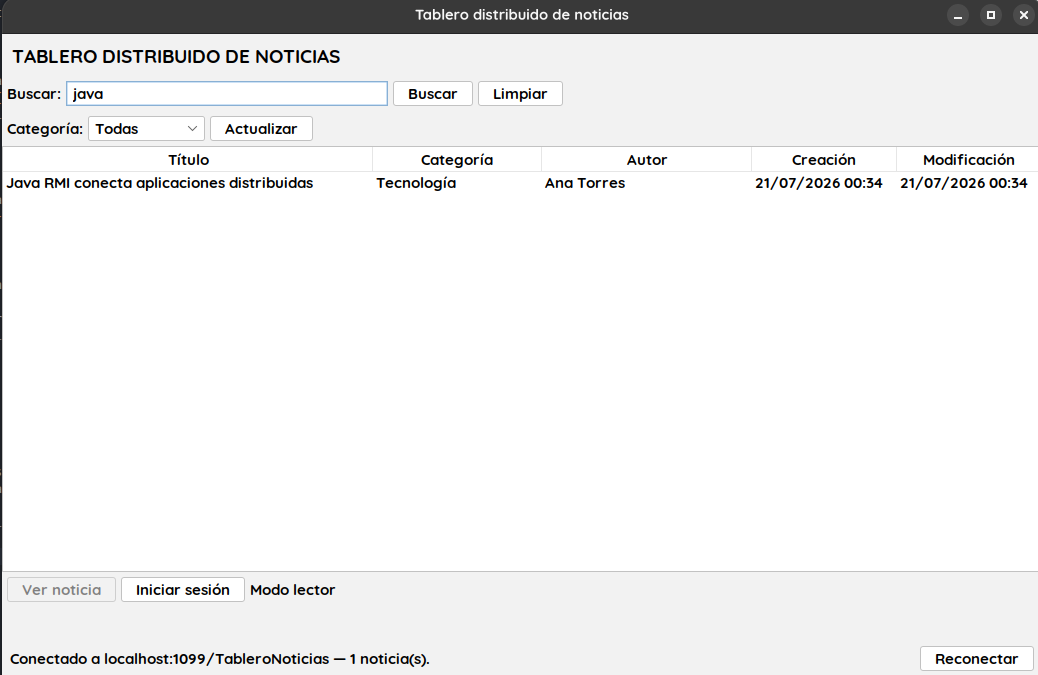
\includegraphics[width=0.8\textwidth]{assets/img/cliente/busqueda-tablero.png}
    \caption{Ventana de búsqueda de noticias en el tablero}
    \label{fig:cliente-ventana-busqueda}
\end{figure}

Para que un usuario pueda publicar una noticia, debe iniciar sesión con un usuario registrado. Para ello solo presiona el botón \emph{Iniciar sesión} y se muestra la ventana de inicio de sesión, como se aprecia en la Figura \ref{fig:cliente-ventana-login}. En esta ventana el usuario debe ingresar su nombre de usuario y contraseña para poder iniciar sesión.

\begin{figure}[H]
    \centering
    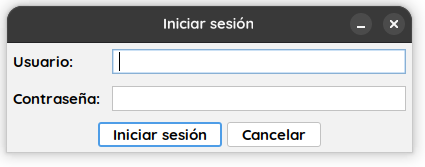
\includegraphics[width=0.4\textwidth]{assets/img/cliente/inicio-sesion.png}
    \caption{Ventana de inicio de sesión del cliente}
    \label{fig:cliente-ventana-login}
\end{figure}

Si el usuario ingresa las credenciales incorrectas se muestra un mensaje de error, como se aprecia en la Figura \ref{fig:cliente-ventana-error-login}. En este caso, el usuario debe verificar sus credenciales y volver a intentar iniciar sesión.